\newpage
\section{実験結果}
選定したシナリオ 28 例中,24 例の自律移動を確認した.
\tabref{tab:scenario_result}に全シナリオの走行の可否を示す.
また, 1 例として Scenario35 を走行時の実験の様子を\figref{fig:exp_path}に示す.

\begin{table}[]
    \centering
    \caption{Results of the scenario-based navigation}\label{tab:scenario_result}
    \begin{tabular}{|c|c|}
    \hline
    scenario & success or failure \\ \hline
    1        & ○                  \\ \hline
    3        & ×                  \\ \hline
    4        & ×                  \\ \hline
    5        & ○                  \\ \hline
    6        & ○                  \\ \hline
    9        & ×                  \\ \hline
    20       & ○                  \\ \hline
    21       & ○                  \\ \hline
    22       & ○                  \\ \hline
    24       & ○                  \\ \hline
    25       & ○                  \\ \hline
    27       & ○                  \\ \hline
    28       & ○                  \\ \hline
    29       & ○                  \\ \hline
    30       & ○                  \\ \hline
    31       & ○                  \\ \hline
    32       & ○                  \\ \hline
    33       & ○                  \\ \hline
    34       & ×                  \\ \hline
    35       & ○                  \\ \hline
    36       & ○                  \\ \hline
    37       & ○                  \\ \hline
    38       & ○                  \\ \hline
    39       & ○                  \\ \hline
    40       & ○                  \\ \hline
    41       & ○                  \\ \hline
    42       & ○                  \\ \hline
    50       & ○                  \\ \hline
    \end{tabular}
\end{table}

\begin{figure*}[htbp]
    \begin{tabular}{ccc}
        \begin{minipage}[t]{0.5\textwidth}
            \centering
            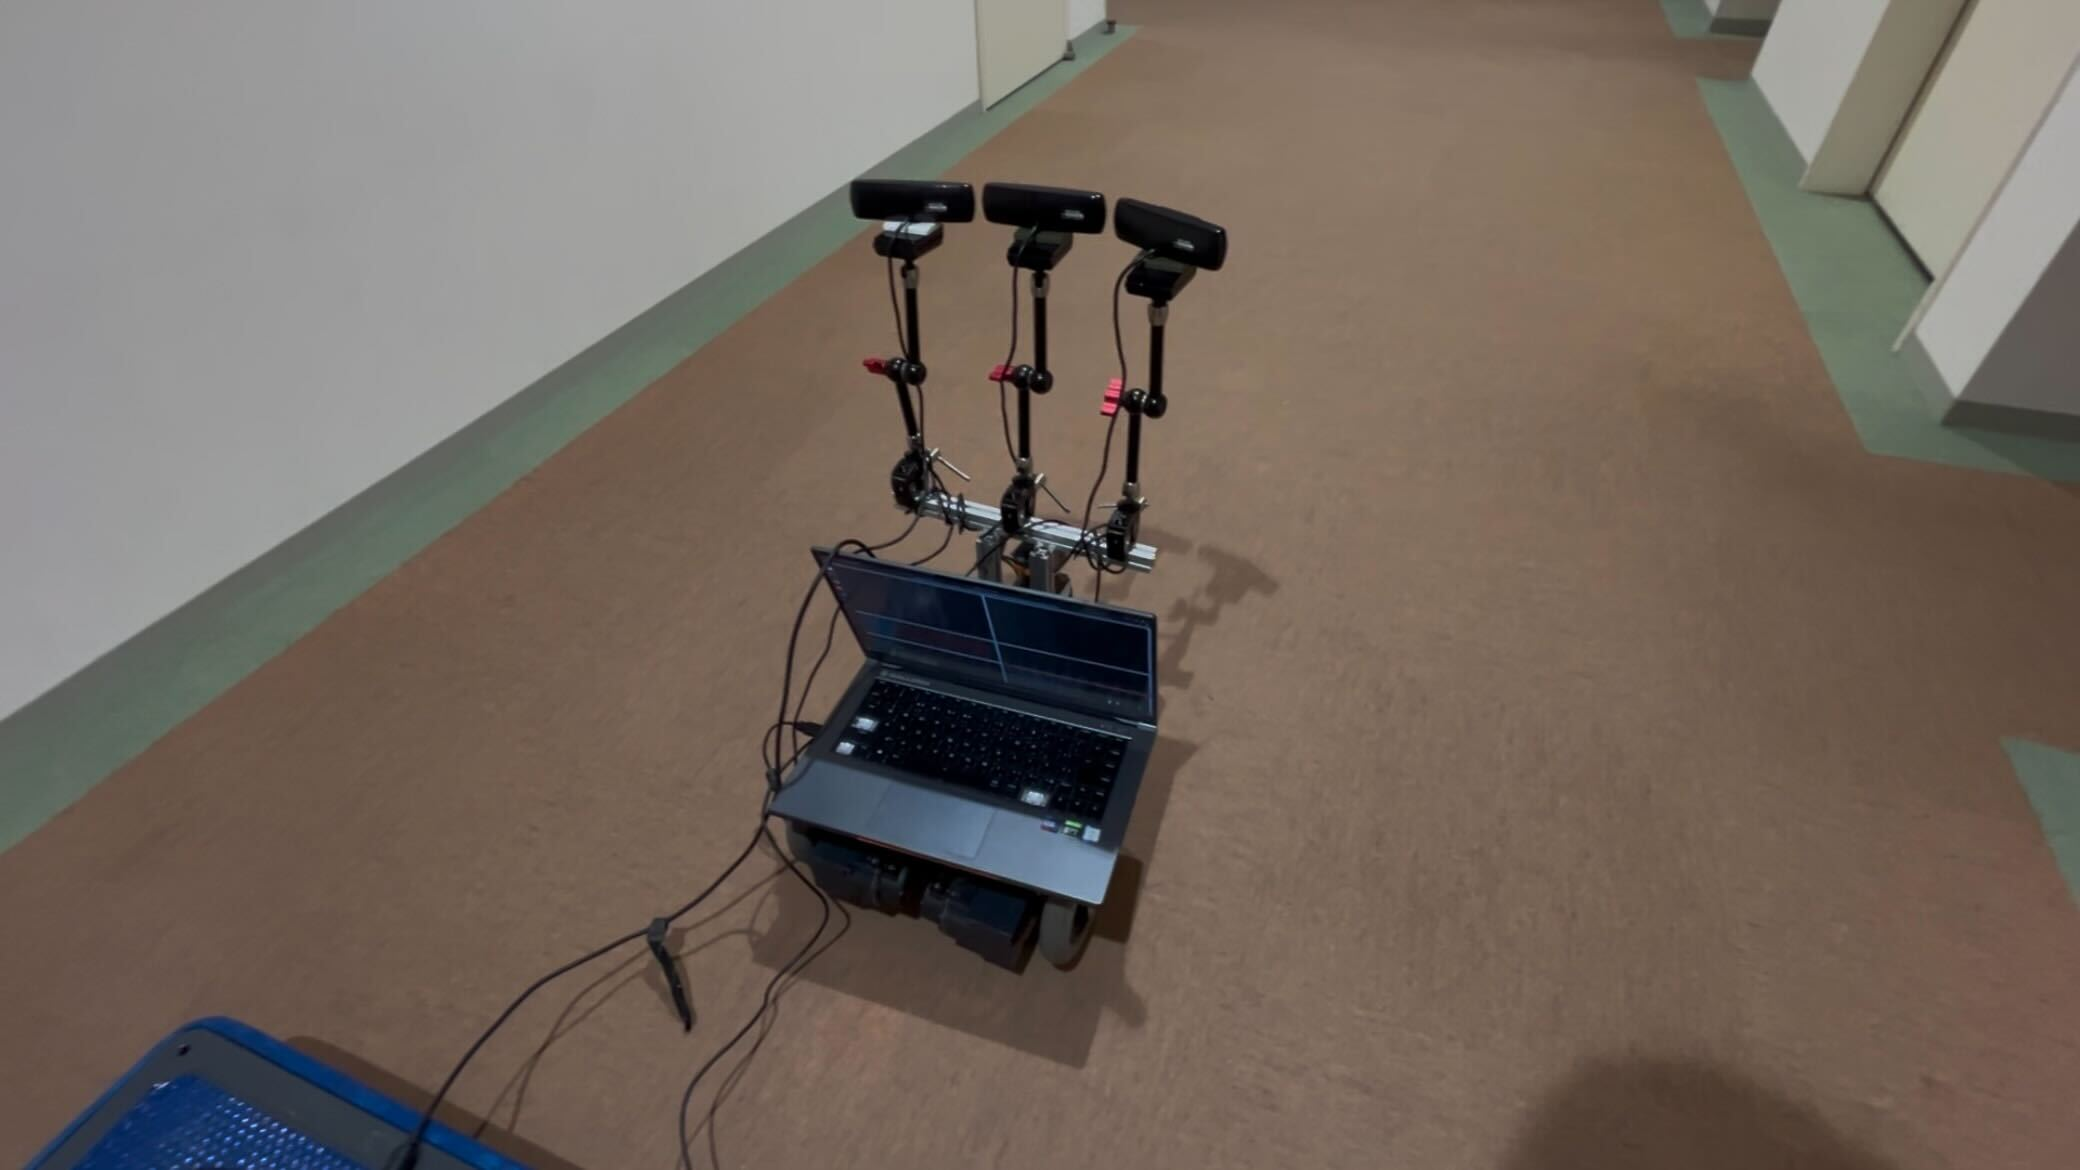
\includegraphics[keepaspectratio, width=55mm]{images/png/ishiguro/exp_0.png}
            \subcaption{突き当たりまで直進}
        \end{minipage} &
        \begin{minipage}[t]{0.5\textwidth}
            \centering
            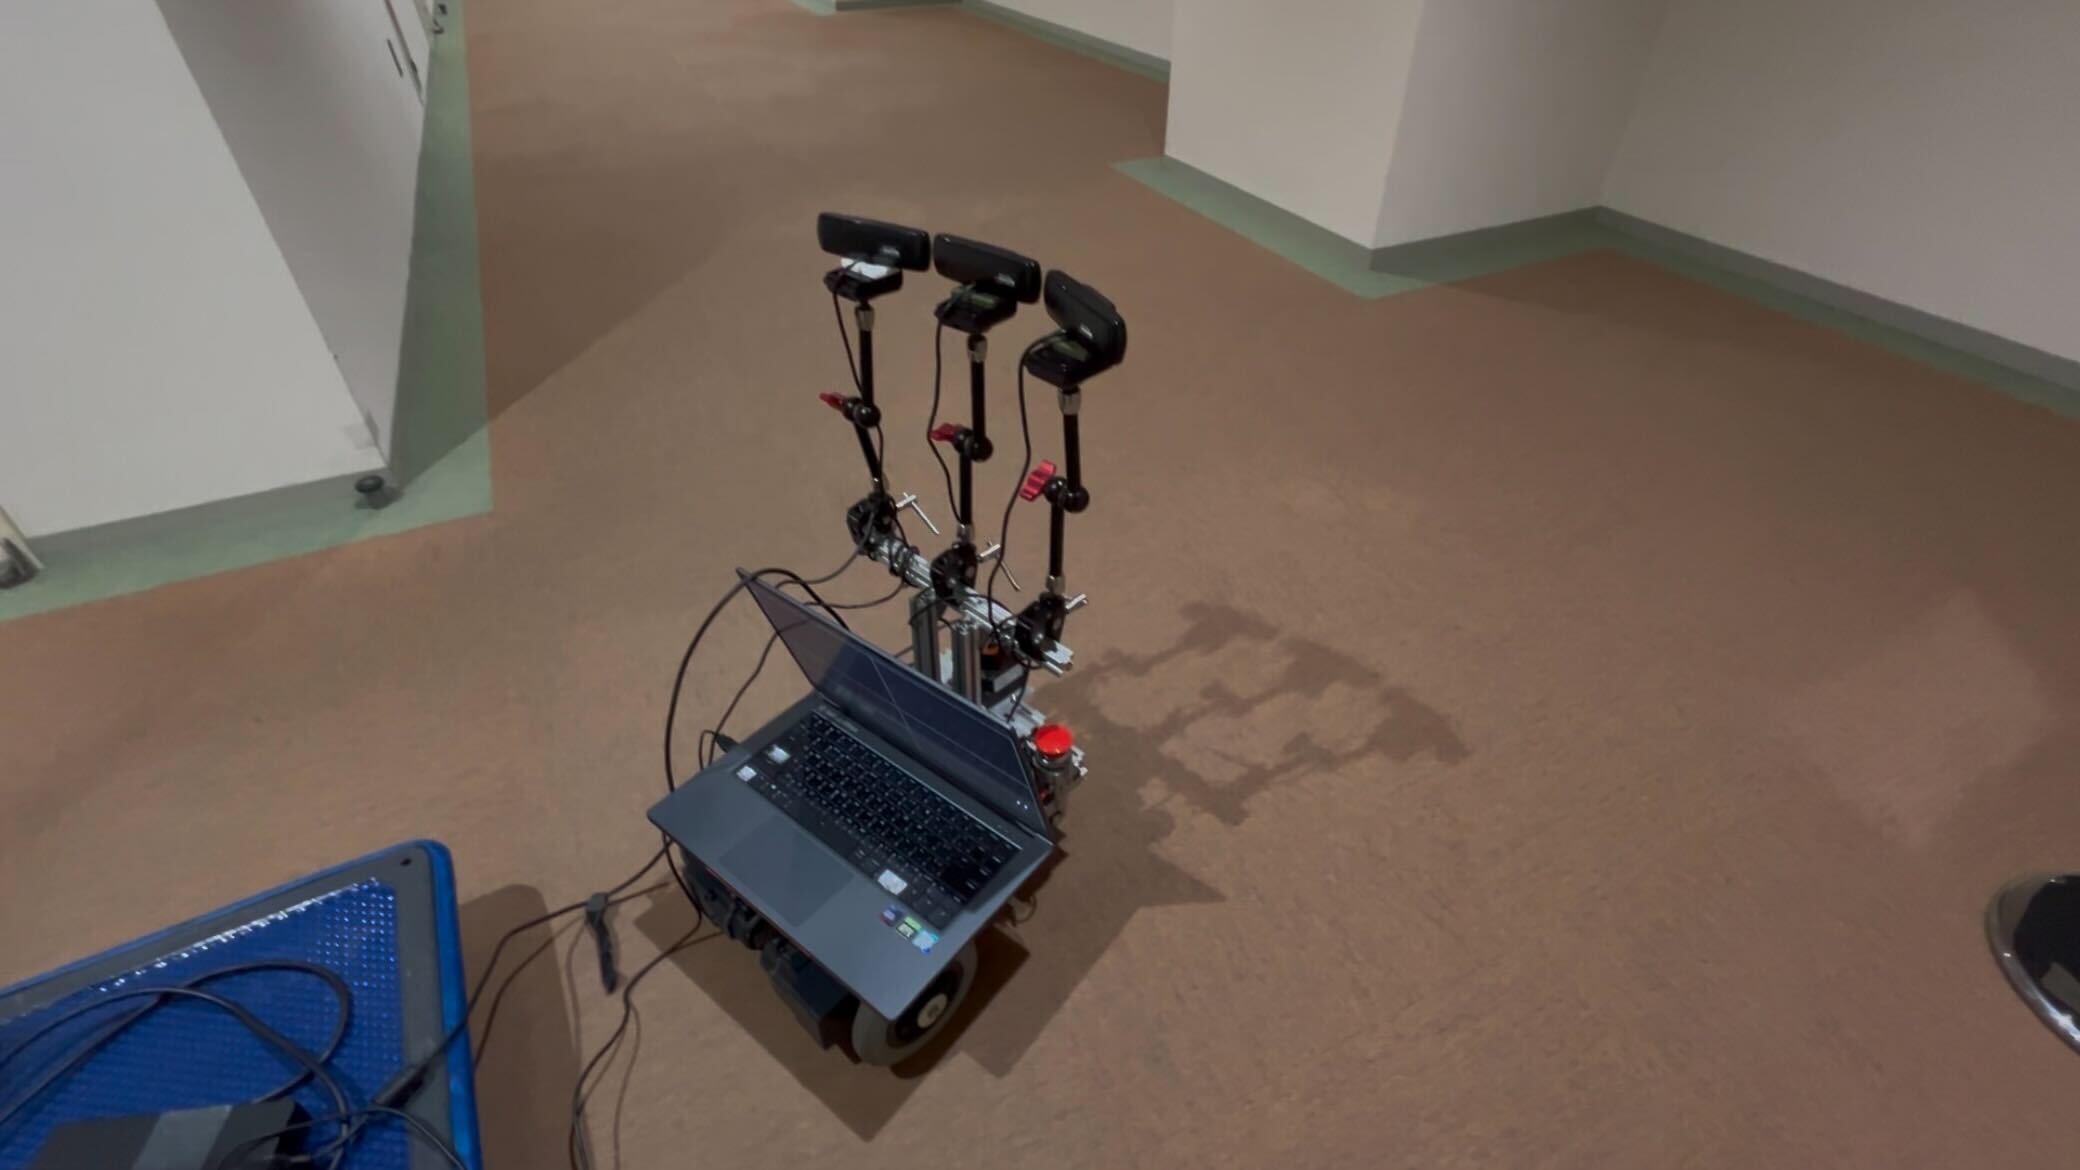
\includegraphics[keepaspectratio, width=55mm]{images/png/ishiguro/exp_1.png}
            \subcaption{左折}
        \end{minipage} \\
        \begin{minipage}[t]{0.5\textwidth}
            \centering
            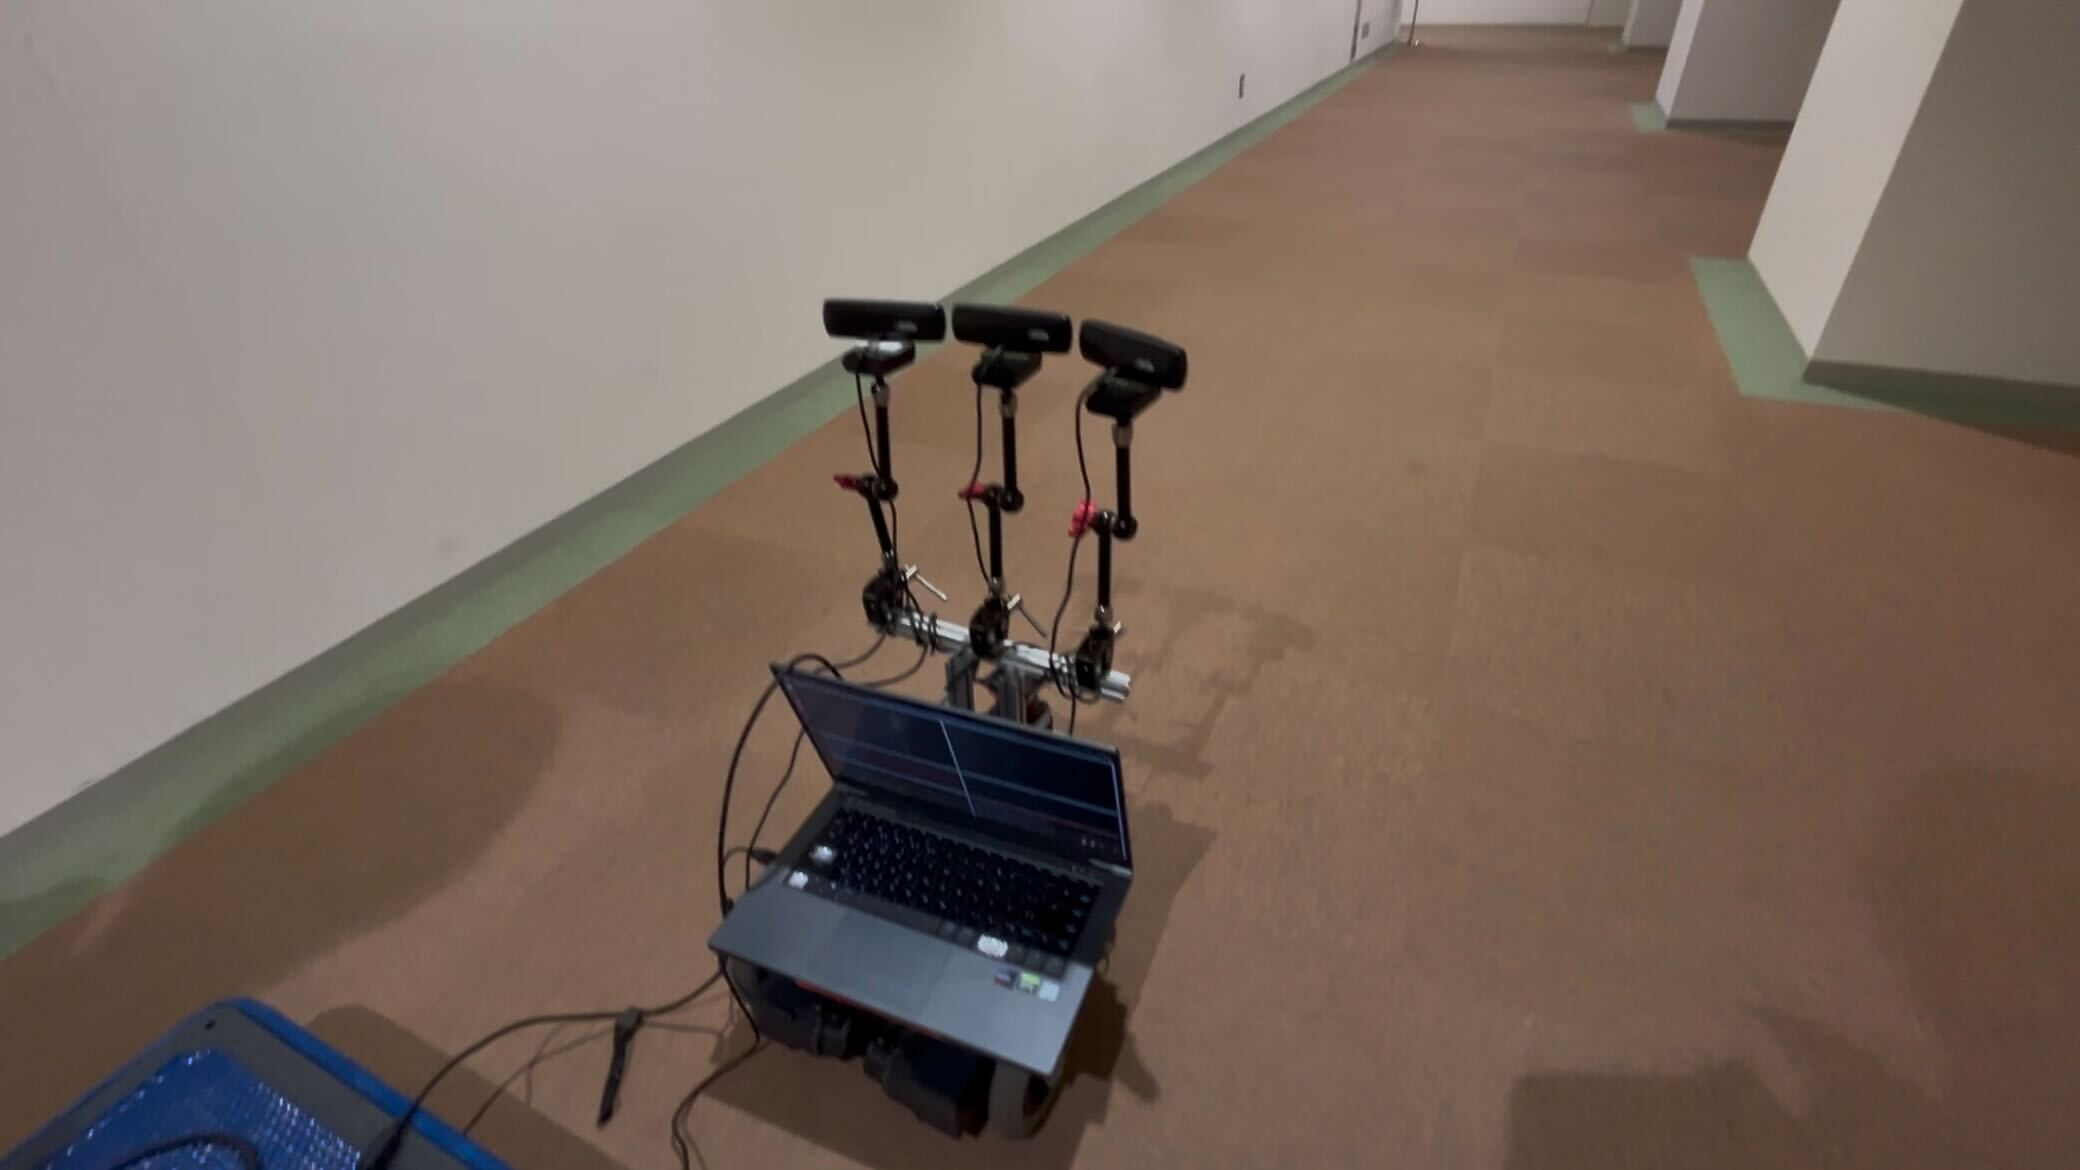
\includegraphics[keepaspectratio, width=55mm]{images/png/ishiguro/exp_2.png}
            \subcaption{突き当たりまで直進}
        \end{minipage} &
        \begin{minipage}[t]{0.5\textwidth}
            \centering
            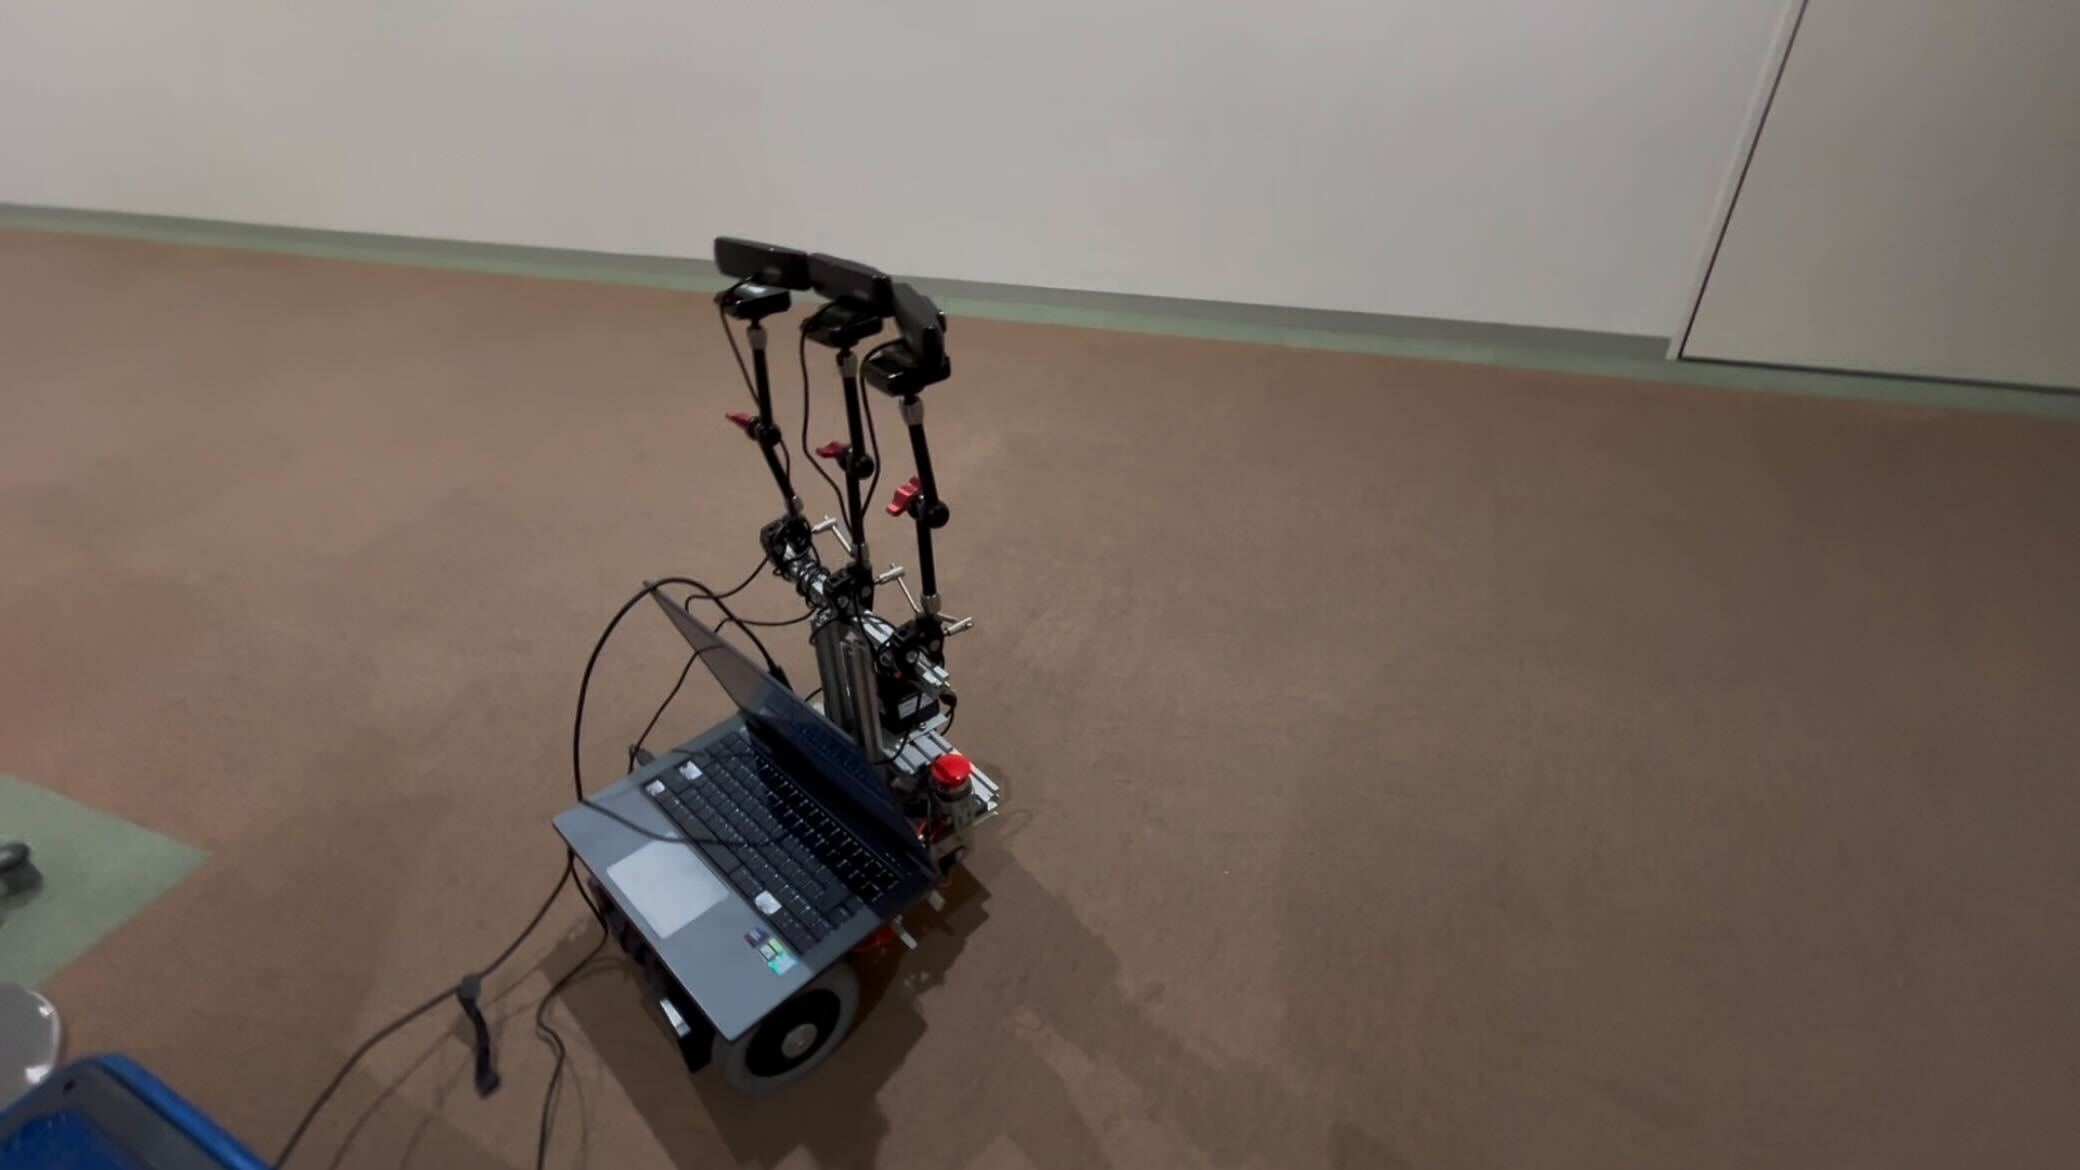
\includegraphics[keepaspectratio, width=55mm]{images/png/ishiguro/exp_3.png}
            \subcaption{右折}
        \end{minipage} \\
        \begin{minipage}[t]{0.5\textwidth}
            \centering
            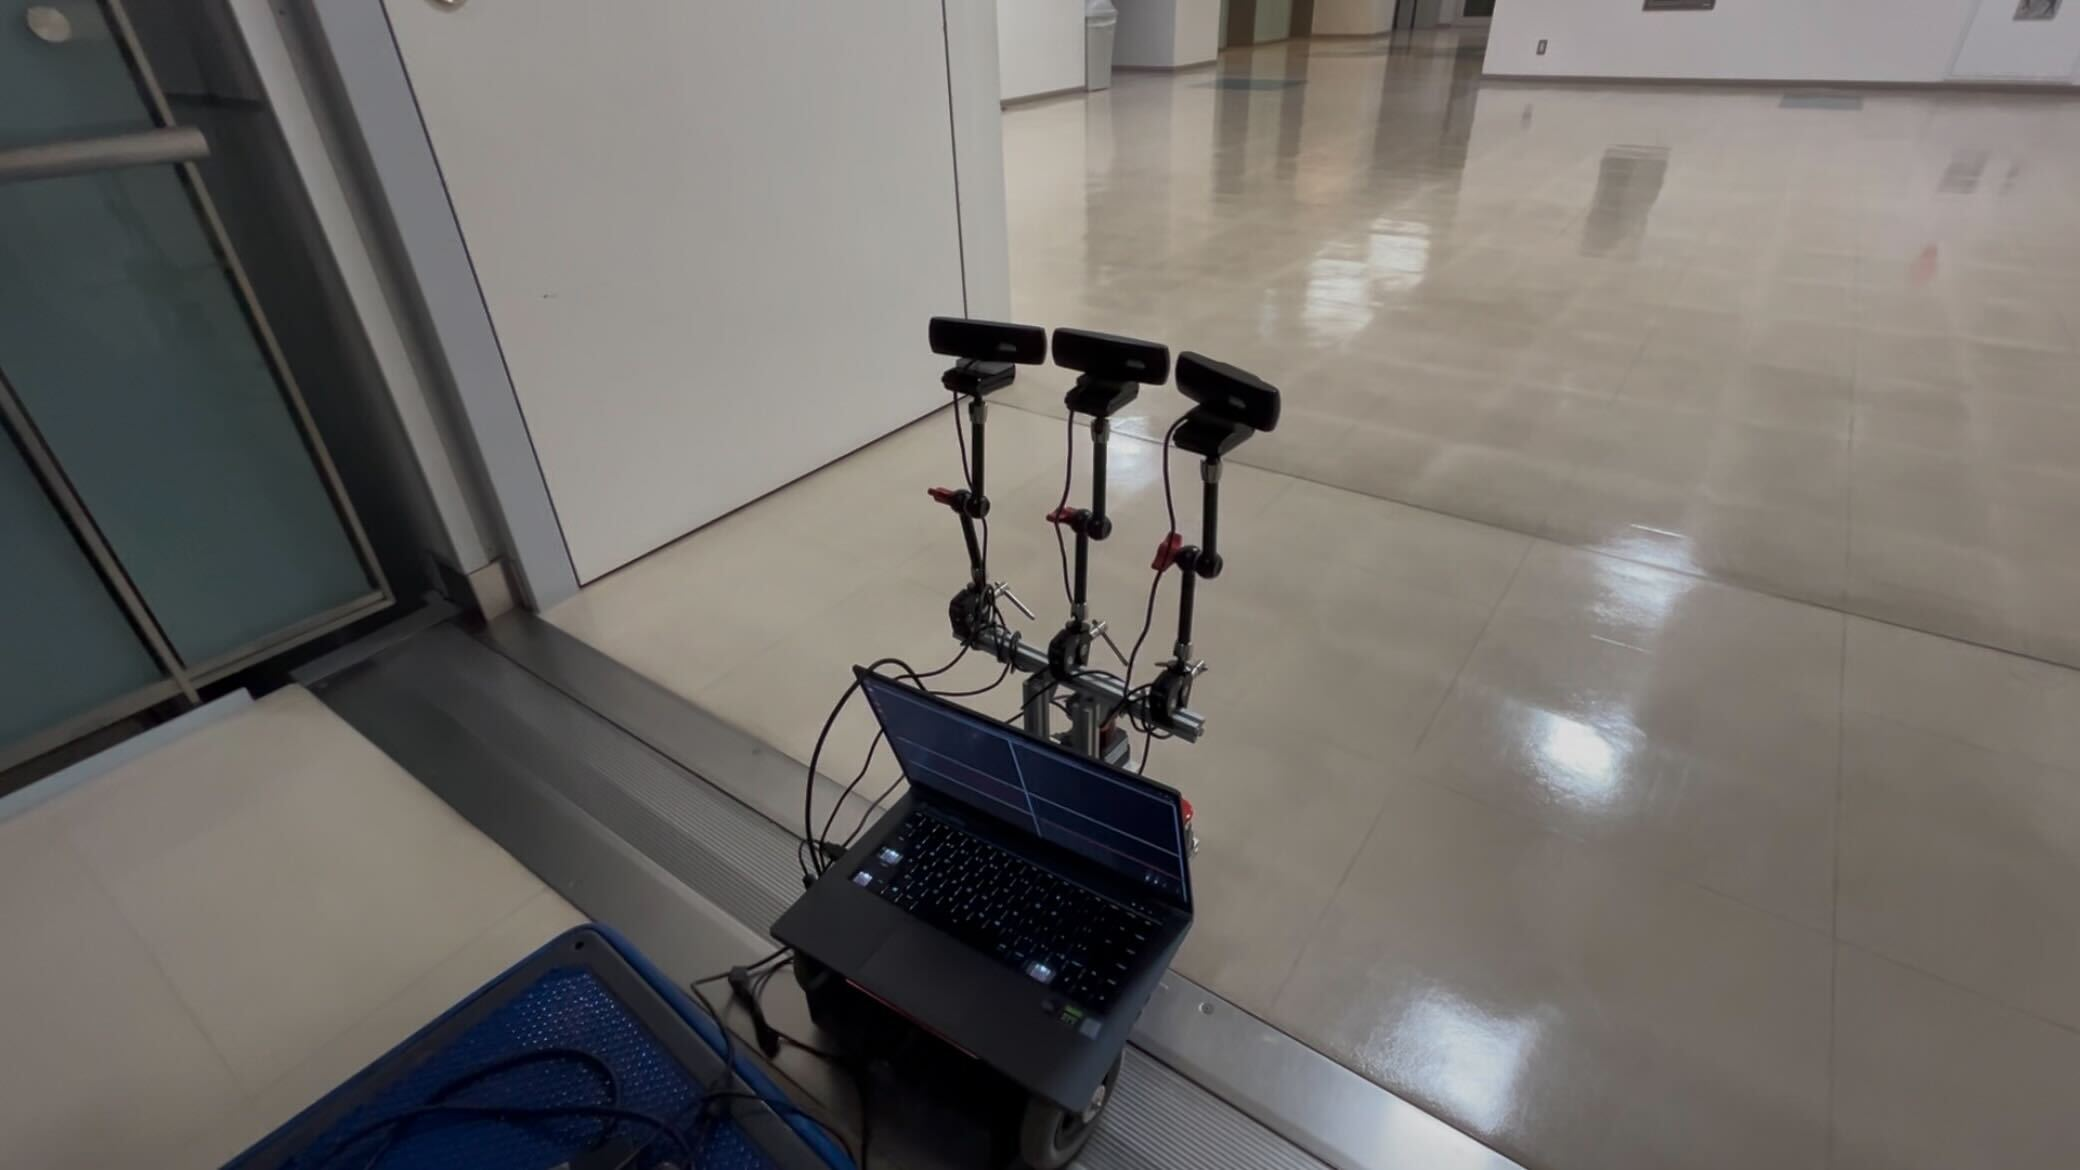
\includegraphics[keepaspectratio, width=55mm]{images/png/ishiguro/exp_4.png}
            \subcaption{突き当たりまで直進}
        \end{minipage} &
        \begin{minipage}[t]{0.5\textwidth}
            \centering
            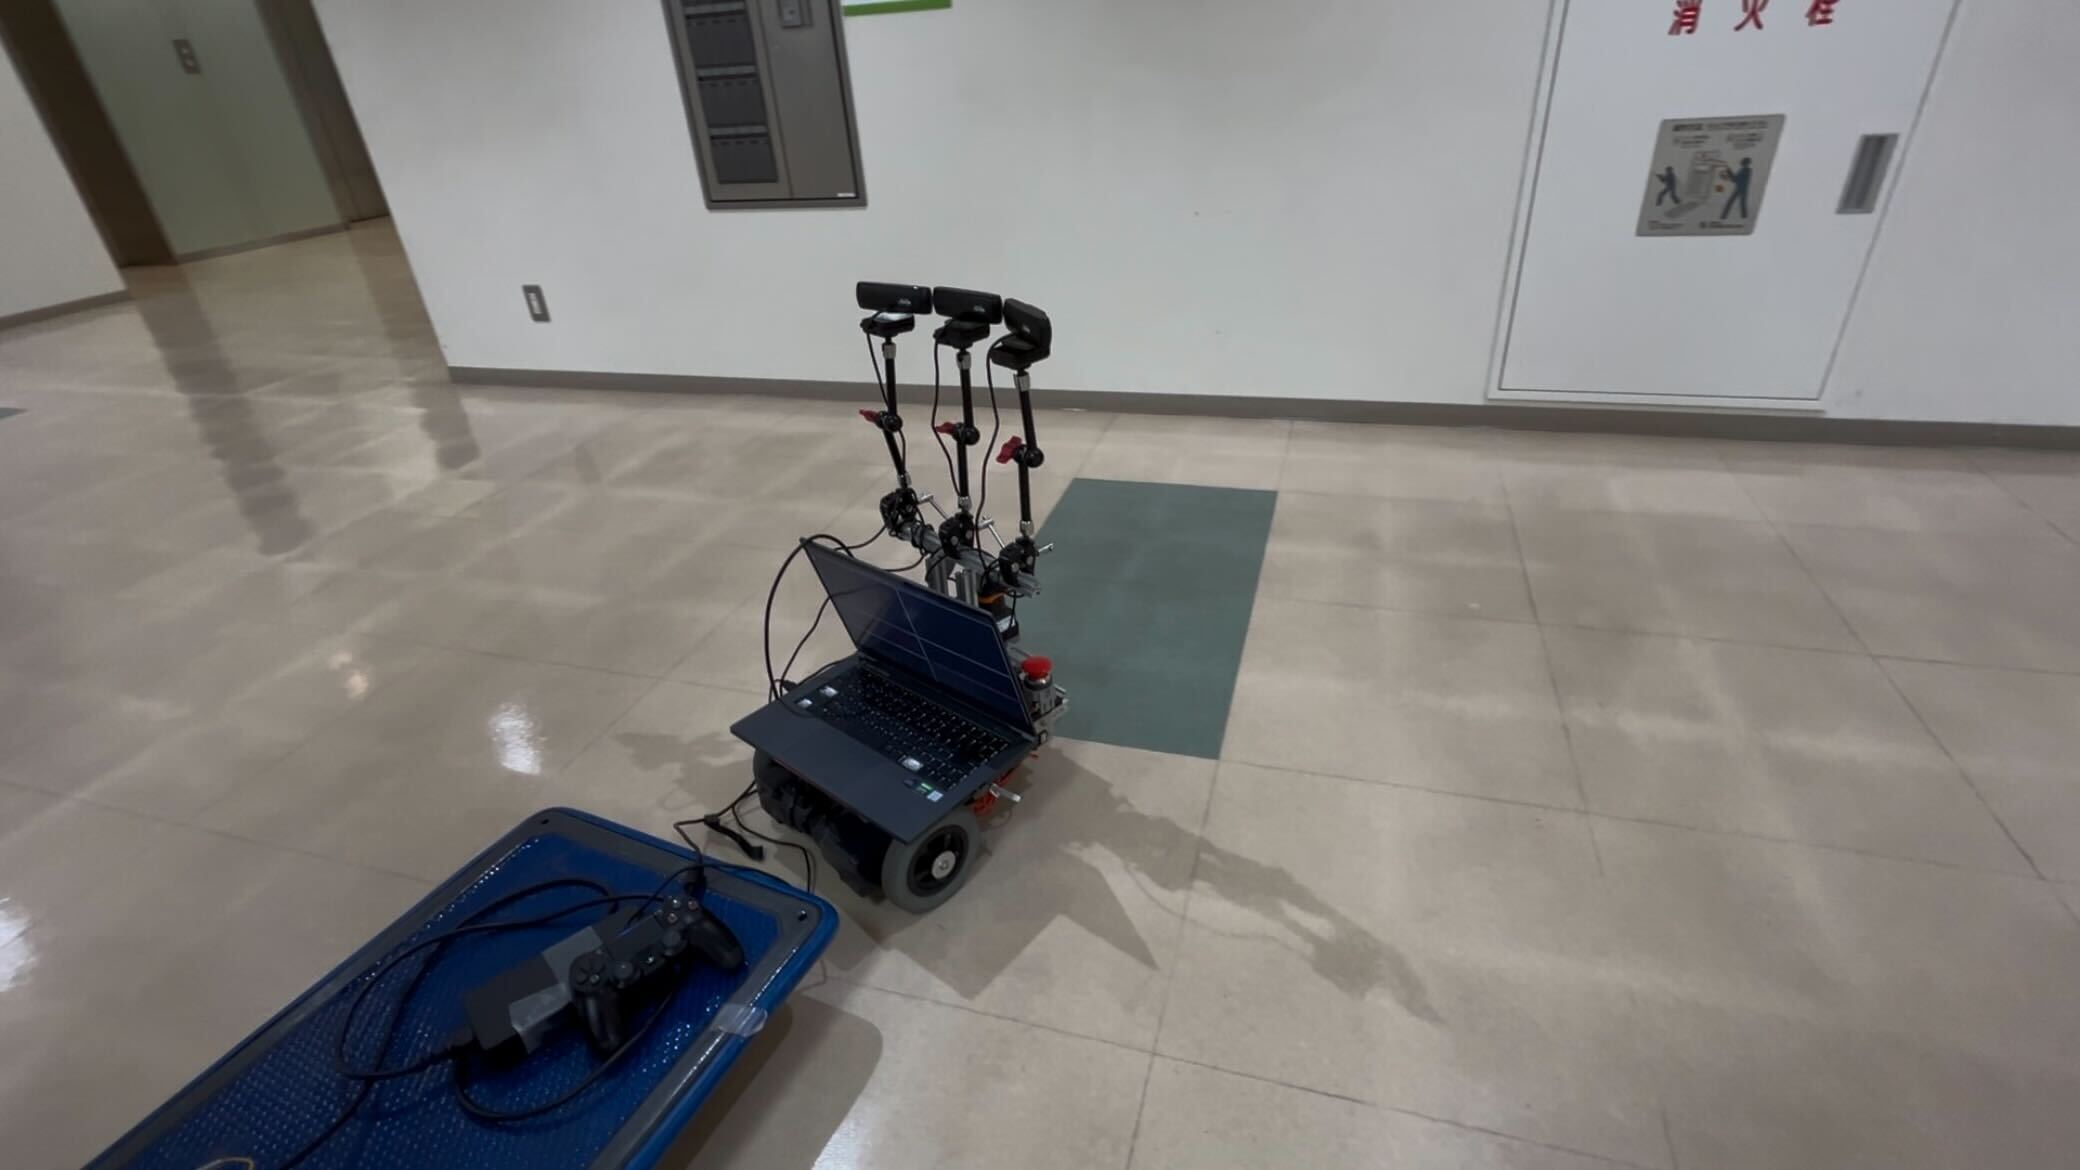
\includegraphics[keepaspectratio, width=55mm]{images/png/ishiguro/exp_5.png}
            \subcaption{右折}
        \end{minipage} \\
        \begin{minipage}[t]{0.5\textwidth}
            \centering
            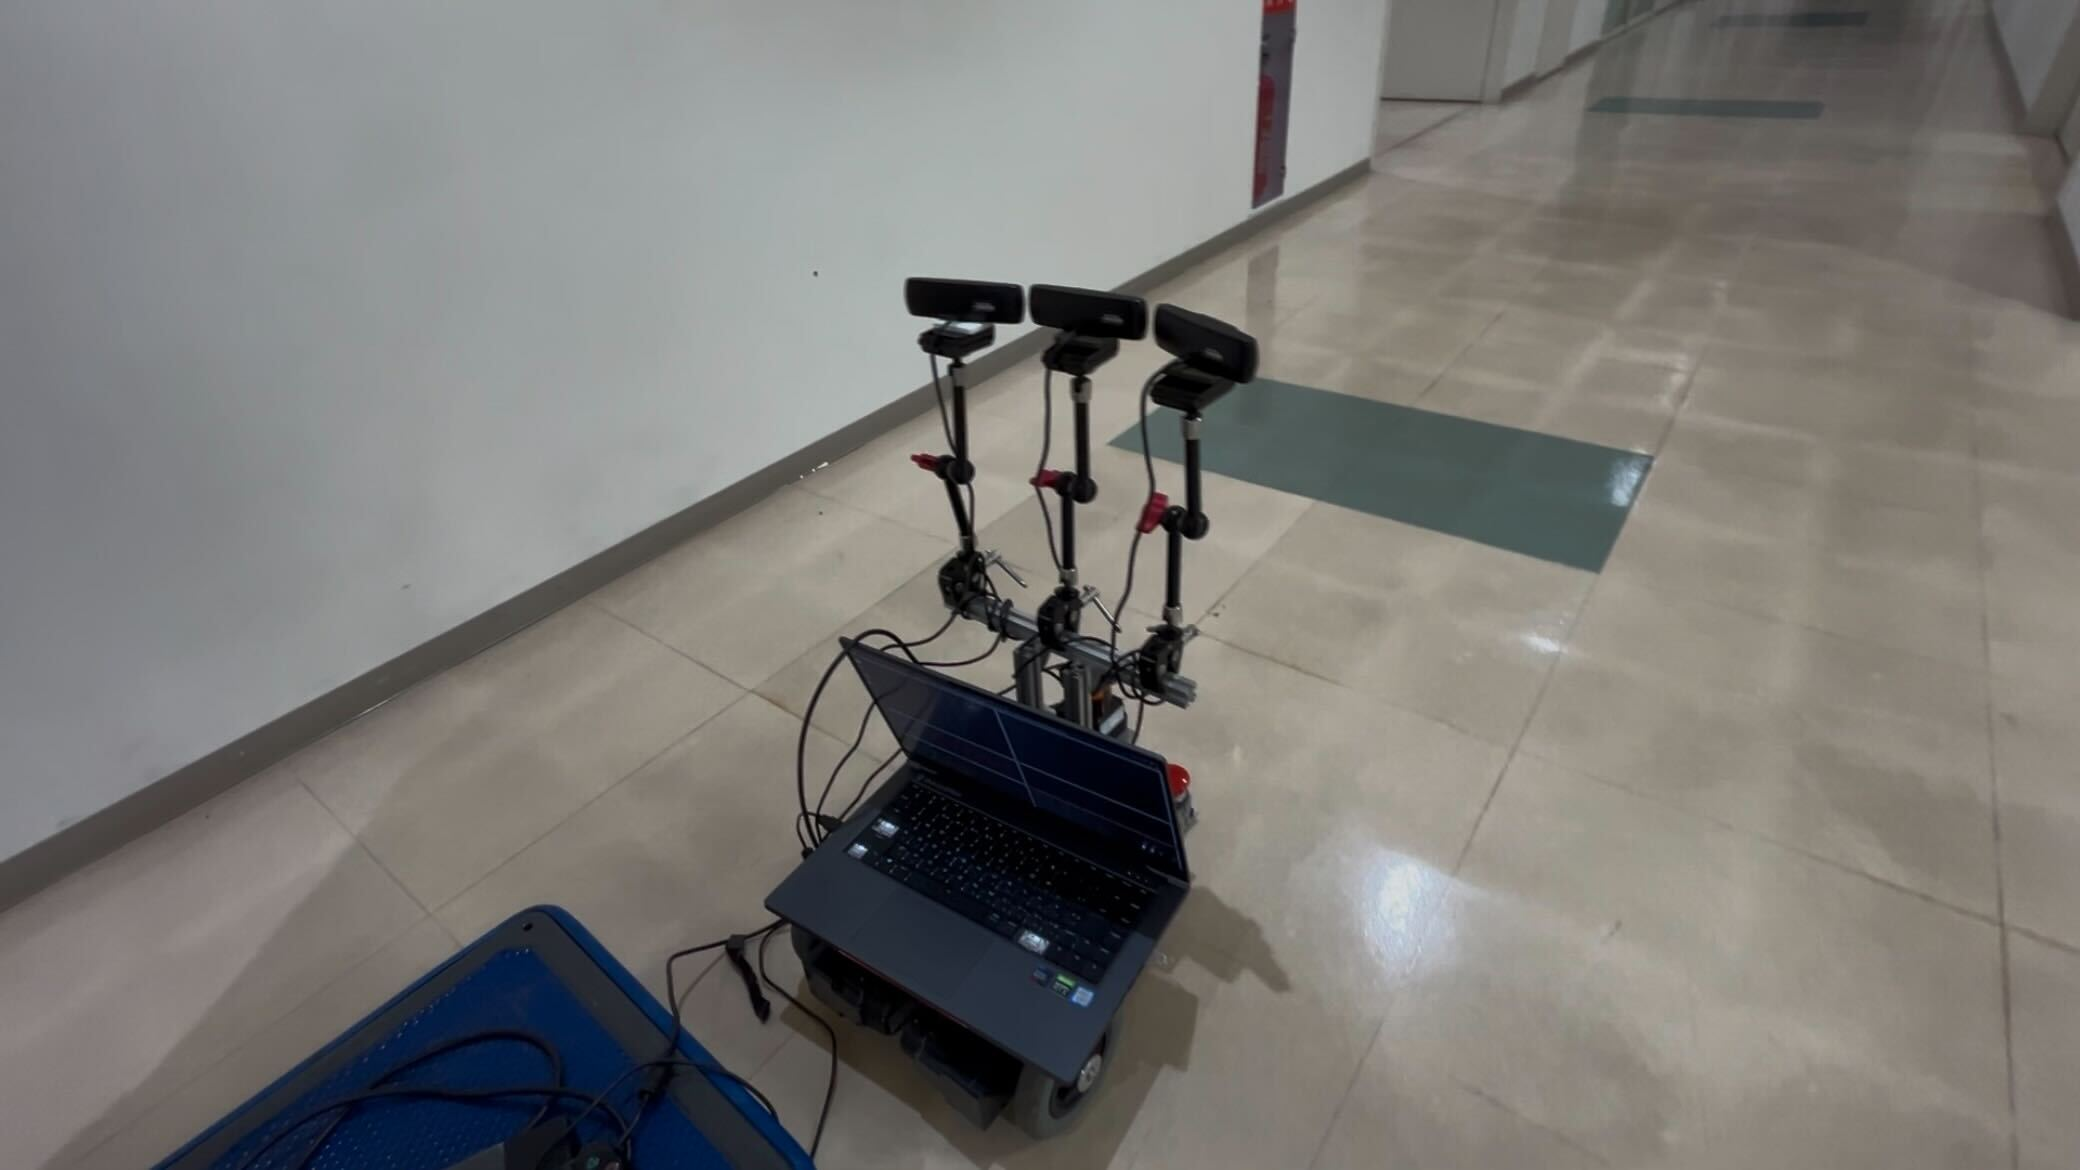
\includegraphics[keepaspectratio, width=55mm]{images/png/ishiguro/exp_6.png}
            \subcaption{次の角まで直進}
        \end{minipage} &
        \begin{minipage}[t]{0.5\textwidth}
            \centering
            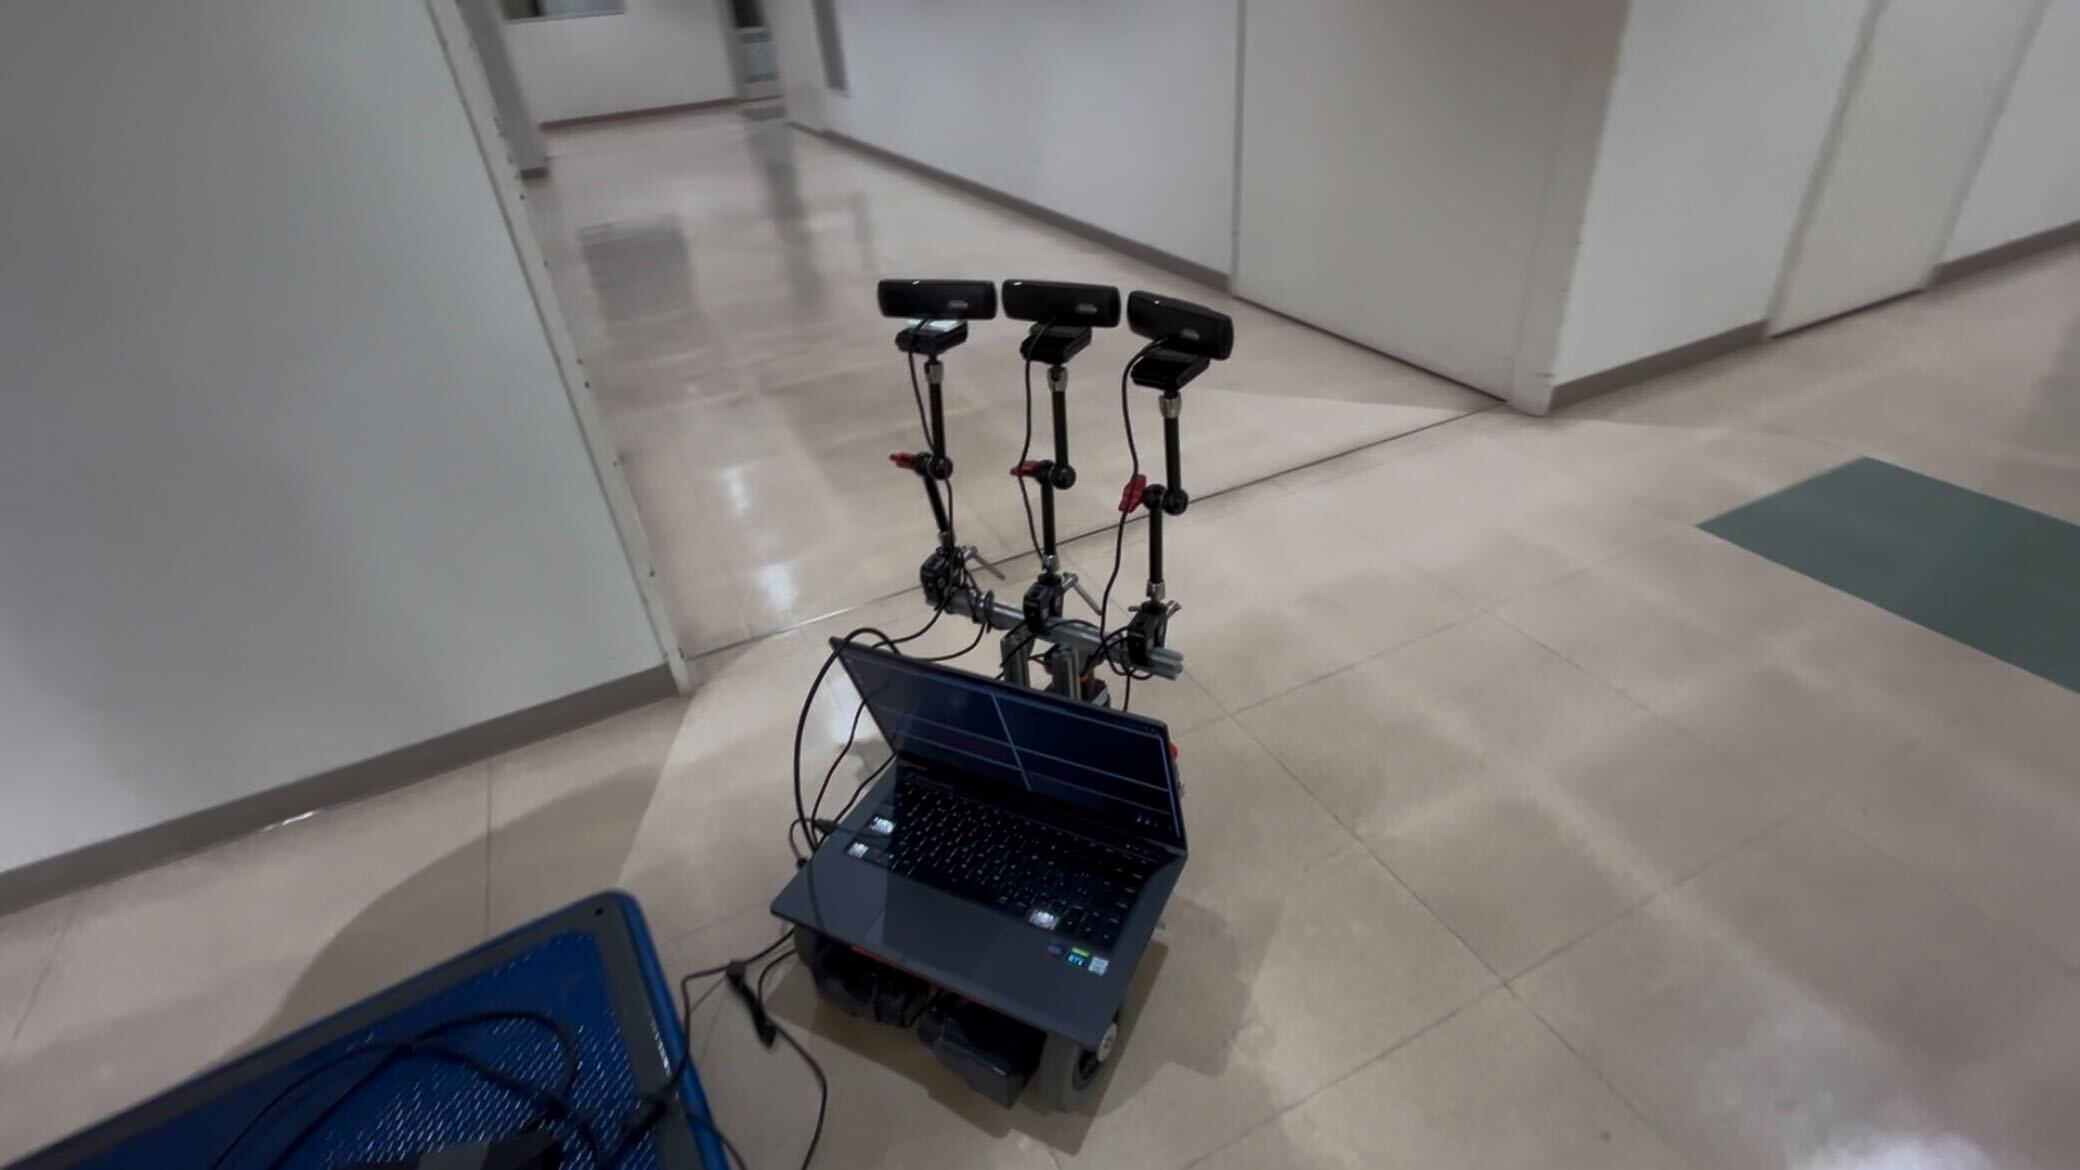
\includegraphics[keepaspectratio, width=55mm]{images/png/ishiguro/exp_7.png}
            \subcaption{左折}
        \end{minipage} \\
        \begin{minipage}[t]{0.5\textwidth}
            \centering
            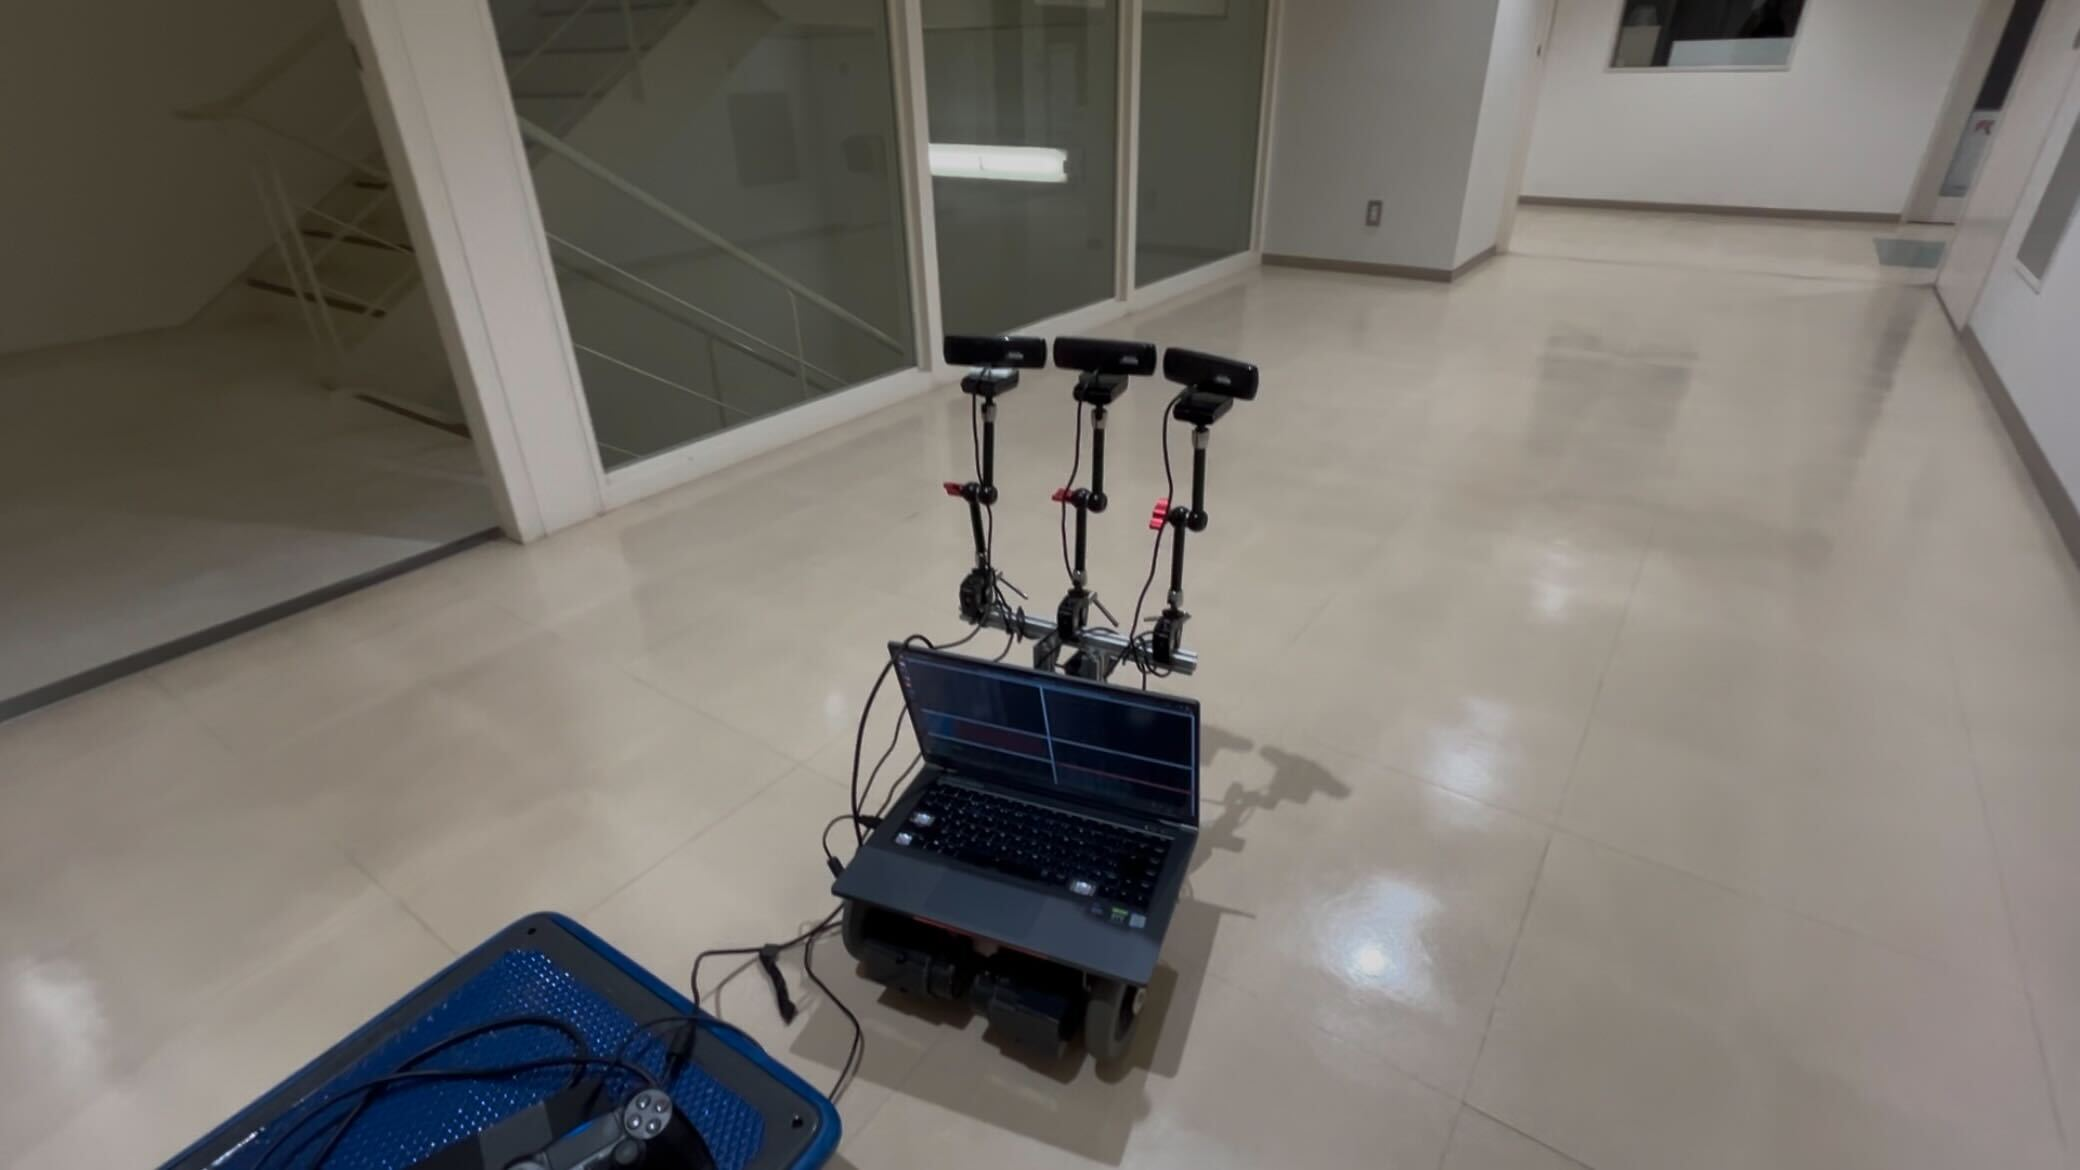
\includegraphics[keepaspectratio, width=55mm]{images/png/ishiguro/exp_8.png}
            \subcaption{突き当たりまで直進}
        \end{minipage} &
        \begin{minipage}[t]{0.5\textwidth}
            \centering
            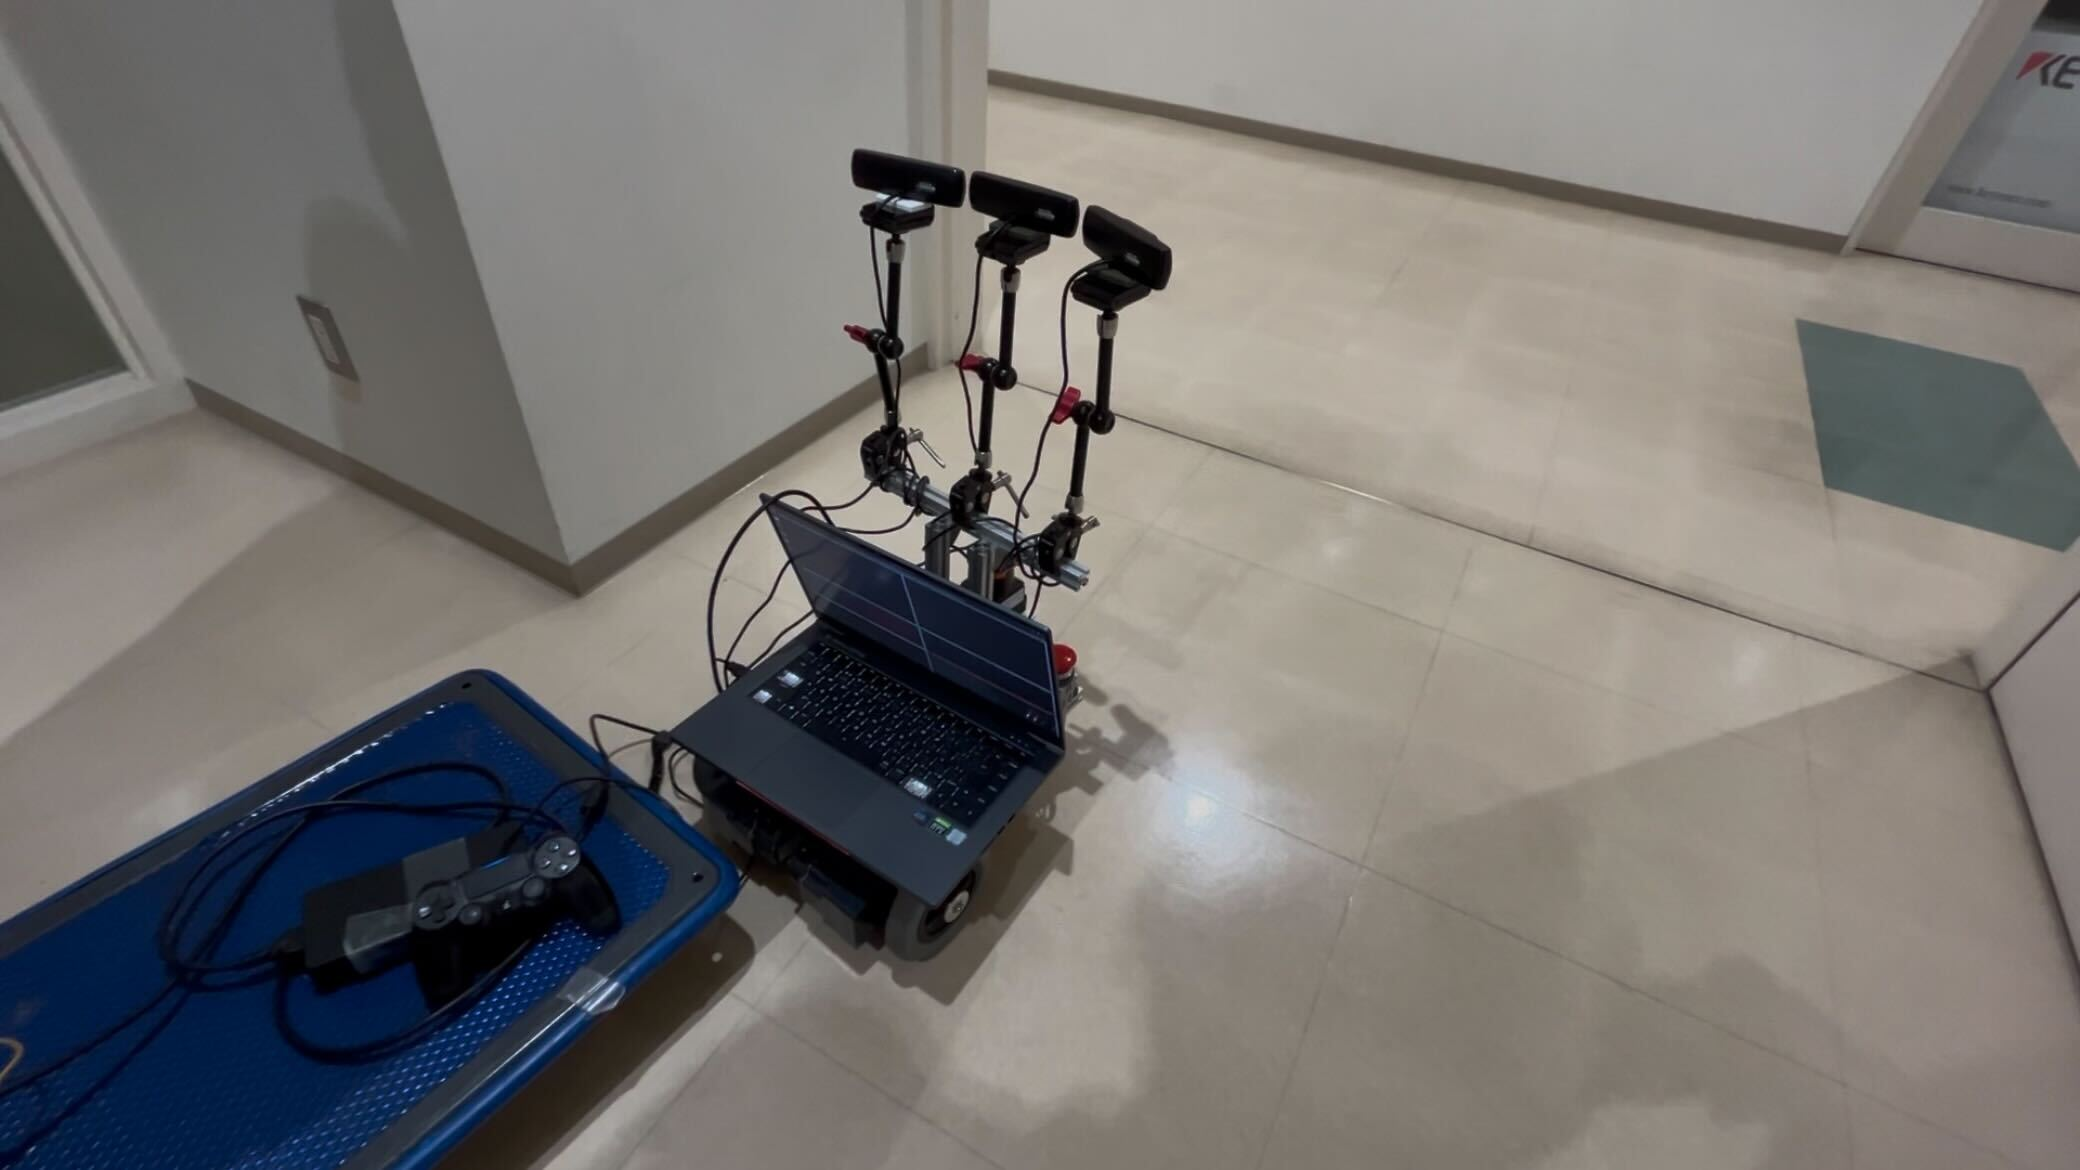
\includegraphics[keepaspectratio, width=55mm]{images/png/ishiguro/exp_9.png}
            \subcaption{停止}
        \end{minipage}
    \end{tabular}
\caption{An example of the robot applied the proposed system}
\label{fig:exp_path}
\end{figure*}

先行研究で走行が確認されていないエリアでも,経路追従することが確認できた.
また,ロボットがシナリオの道順に沿って,分岐路で適切な経路を選択する様子が確認できた.

\newpage
失敗した 4 例ではそれぞれ,曲がり角で左折すべきところを直進した.
\figref{fig:miss}に失敗した箇所を示す.
失敗した 4 例の内訳として,\figref{fig:miss}の青枠に示す失敗が 3 例,緑枠に示す失敗が 1 例となった.
失敗した箇所でも通路の特徴の分類は正しく行われており,経路追従モジュールに与えられる目標方向も正しい値が入力されていた.
失敗の原因をとして,通路分類の結果の切り替わりが遅いことが考えられる.
\figref{fig:mis_1}と\figref{fig:mis_2}に示す画像は失敗箇所において,学習時とテスト時に「左折」の目標方向を与えたタイミングでのロボットの位置である.
学習時は角から 1 ~ 2 m ほど前方で目標方向が与えられているのに対し,テスト時では 角から 0.2 ~ 0.5 m まで近づいてから与えられていることがわかった.
経路追従モジュールに目標方向が与えられるタイミングは,通路分類の結果が変わったタイミングとなる.
つまり通路分類が遅れることで目標方向が与えるタイミングが学習時より遅くなり,左折できないと考えた.
確認として,学習時と同じタイミングで経路追従モジュールに目標方向を与えた場合,左折する様子が確認できた.
このことから,失敗要因として通路分類の切り替わりが遅いことが考えられる.

\begin{figure}[htbp]
    \centering
    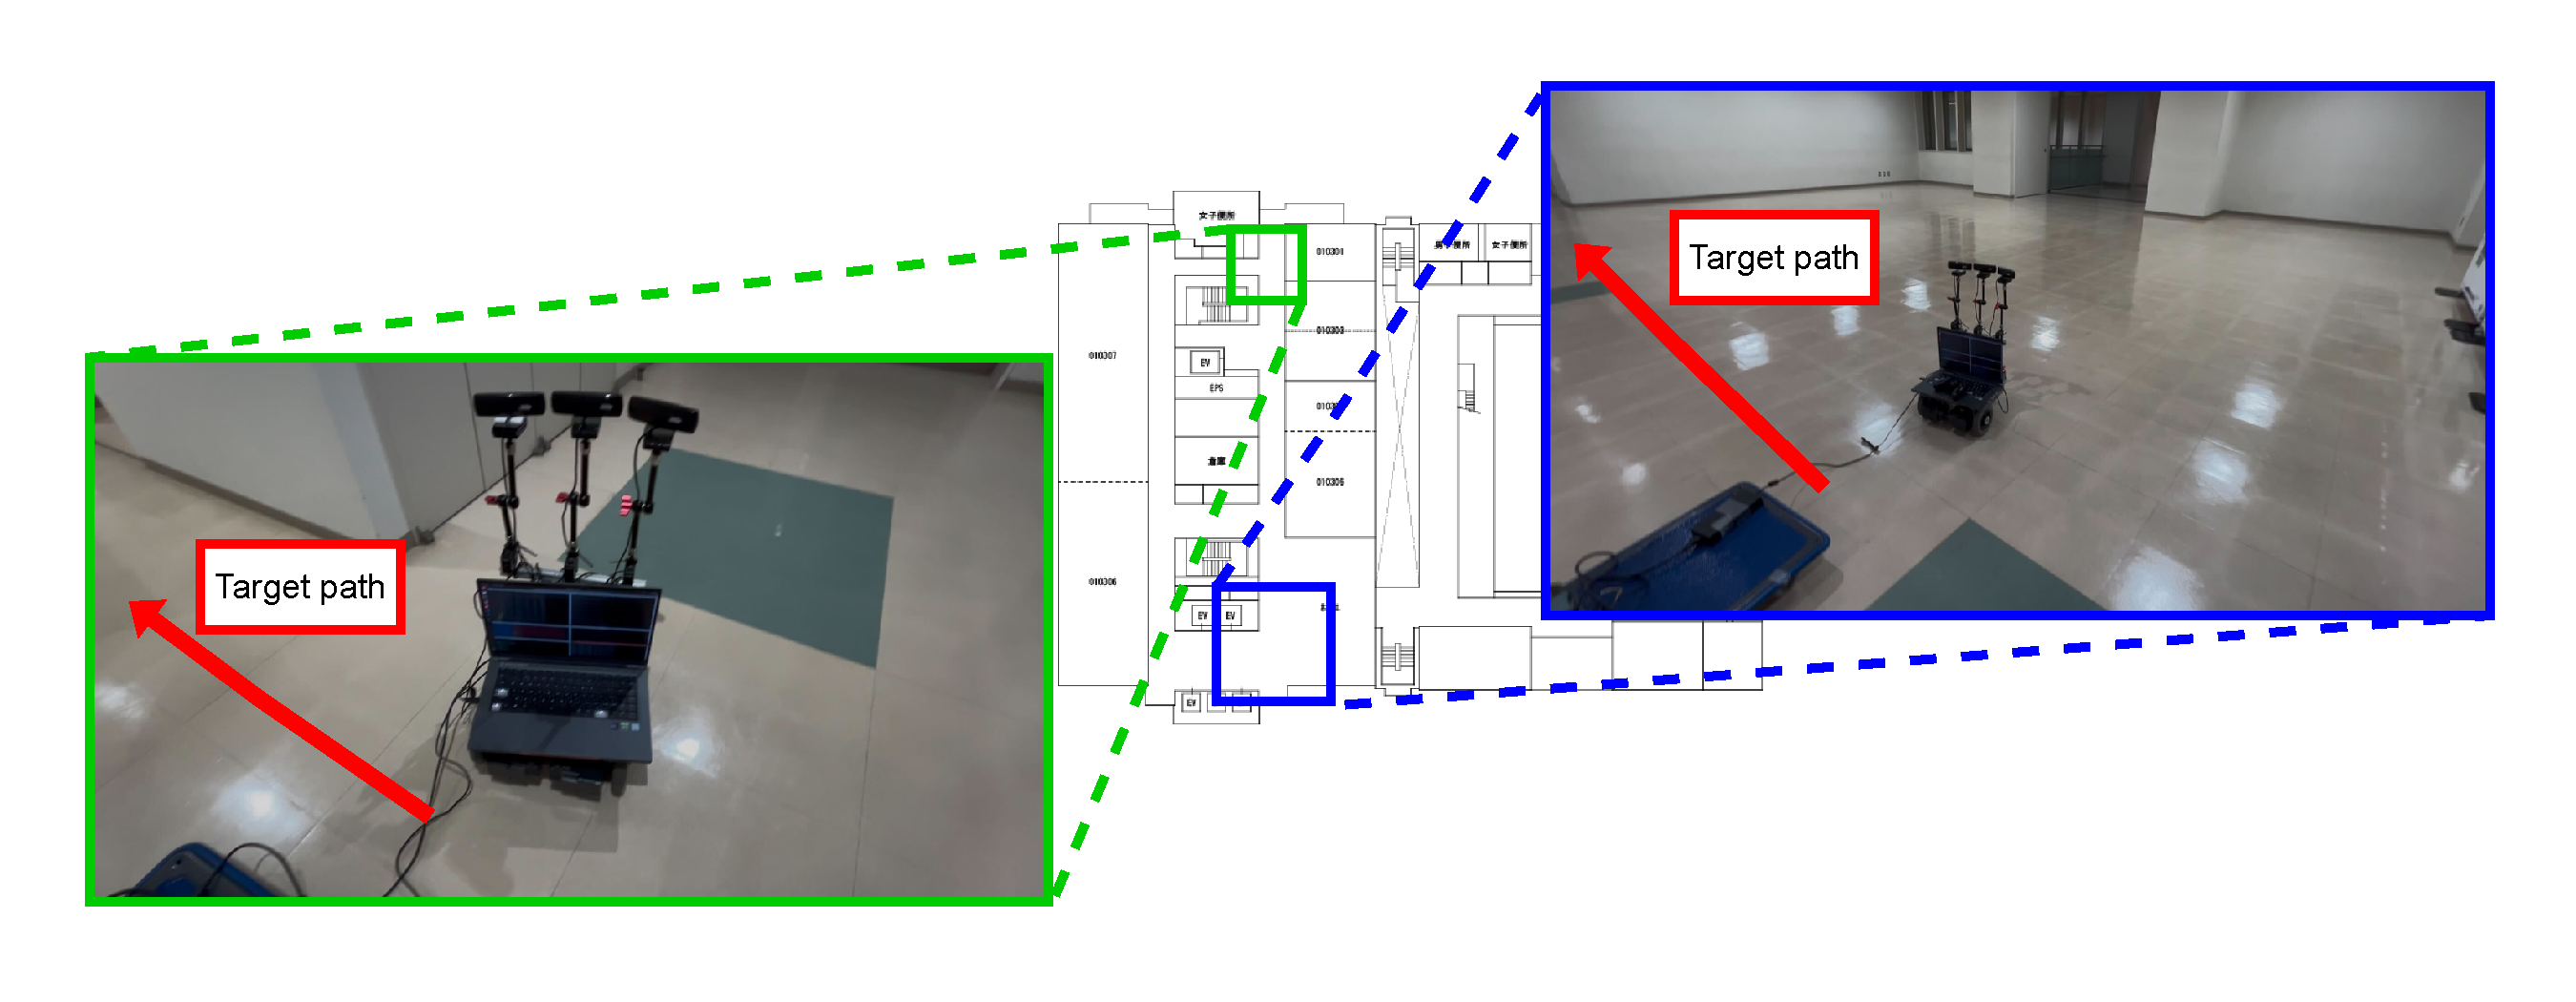
\includegraphics[width=130mm]{images/pdf/ishiguro/miss.pdf}
    \caption{Failed place}
    \label{fig:miss}
\end{figure}

\clearpage

\begin{figure*}[htbp]
    \begin{tabular}{ccc}
        \begin{minipage}[t]{0.5\textwidth}
            \centering
            \includegraphics[keepaspectratio, width=70mm]{images/png/ishiguro/learning_1.png}
            \subcaption{Location of label changes during learning}
        \end{minipage} &
        \begin{minipage}[t]{0.5\textwidth}
            \centering
            \includegraphics[keepaspectratio, width=70mm]{images/png/ishiguro/test_1.png}
            \subcaption{Location of label changes during testing}
        \end{minipage}
    \end{tabular}
\caption{Failure point 1}
\label{fig:mis_1}
\end{figure*}

\begin{figure*}[htbp]
    \begin{tabular}{ccc}
        \begin{minipage}[t]{0.5\textwidth}
            \centering
            \includegraphics[keepaspectratio, width=70mm]{images/png/ishiguro/learning_2.png}
            \subcaption{Location of label changes during learning}
        \end{minipage} &
        \begin{minipage}[t]{0.5\textwidth}
            \centering
            \includegraphics[keepaspectratio, width=70mm]{images/png/ishiguro/test_2.png}
            \subcaption{Location of label changes during testing}
        \end{minipage}
    \end{tabular}
\caption{Failure point 2}
\label{fig:mis_2}
\end{figure*}